\documentclass[a4paper]{article}

% CUSTOM maketitle
\makeatletter
\def\@maketitle{%
  \newpage
  \null
  \vskip 1.em
  \begin{center}%
    \let \footnote \thanks
    {\LARGE \bfseries\@title \par}%
    \vskip 1.em%
      {\large \langCourse \par}%
      {\large \langInstitute \par}%
    \vskip 1.em%
      {\large
        \lineskip .5em%
        \begin{tabular}[t]{c}%
          \@author { --- } \@istid \\
          {\href{mailto:\@email}{\tt\@email}}
        \end{tabular}\par}%
    \vskip 1.em%
    \ifx\@coadvisor\undefined
      {\large \langAdvisor: \@advisor \par}%
      \else
      {\large \langAdvisor: \@advisor \par}%
      {\large \langCoadvisor: \@coadvisor \par}%
    \fi

  \end{center}%
  \par
  \vskip 1em}
\makeatother


% Commands to allow defining title, name, etc.
\makeatletter
\newcommand{\@StoreIn}[2]{ \gdef#1{#2} }
\newcommand*{\email}[1]{\@StoreIn{\@email}{#1}}
\newcommand*{\istid}[1]{\@StoreIn{\@istid}{#1\thanks{\langThanks}}}
\newcommand*{\advisor}[1]{\@StoreIn{\@advisor}{#1}}
\newcommand*{\coadvisor}[1]{\@StoreIn{\@coadvisor}{#1}}
\makeatother

% The 'utf8' package contains support for using UTF-8 as input encoding. 
\usepackage[utf8]{inputenc}
% The 'babel' package may correct some hyphenation issues of LaTeX. 
% Select your MAIN LANGUAGE for the Thesis with the 'main=' option.
\usepackage[english,portuguese]{babel}
\usepackage{iflang}
% Language dependent section names
\addto\captionsenglish{
  \renewcommand{\contentsname}{\null ~\vskip 1.em \hfil Contents\hfil}
  \renewcommand{\refname}{Bibliography}
}
\addto\captionsportuguese{
  \renewcommand{\contentsname}{\null ~\vskip 1.em \hfil Conteúdos\hfil}
  \renewcommand{\refname}{Bibliografia}
}

% Solves some font enconding issues related to the output
\usepackage[T1]{fontenc}

% These packages are typically required. 
% Among many other things they add the possibility to put symbols in bold
% by using \boldsymbol (not \mathbf); defines additional fonts and symbols;
% adds the \eqref command for citing equations.
\usepackage{mathtools, amsmath, amsthm, amssymb, amsfonts}
\usepackage{nicefrac}
%

% Tikz  for creating graphics programmatically.
\usepackage{tikz}
\usetikzlibrary{shapes.geometric, arrows, positioning}

% These packages are most usefull for advanced tables. 
% 'multirow' allows to join rows throuhg the command \multirow which works
% similarly with the command \multicolumn.
% The 'colortbl' package allows to color the table (foreground and background)
% The package 'booktabs' provide some additional commands to enhance
% the quality of tables
% The 'longtable' package is only required when tables extend beyond the length
% of one page, which typically does not happen and should be avoided
\usepackage{array}
\usepackage{booktabs}
\usepackage{multirow}
\usepackage{colortbl}
\usepackage{spreadtab}
\usepackage{longtable}
\usepackage{pdflscape}
\usepackage{float}

% Set links for references and citations in document
\usepackage{hyperref}
\hypersetup{ colorlinks=true,
  citecolor=cyan,
  linkcolor=darkgray,
  urlcolor=teal,
  breaklinks=true,
  bookmarksnumbered=true,
  bookmarksopen=true,
}

% Provides better support for handling and breaking URLs.
\usepackage{url}

% The package 'graphicx' supports formats PNG and JPG.
% Package 'subfigure' allows to place figures within figures with own caption. 
% For each of the subfigures use the command \subfigure.
\usepackage{graphicx}
\usepackage[hang,small,bf,tight]{subfigure}

\usepackage[format=hang,labelfont=bf,font=small]{caption}
% the following customization adds vertical space between caption and the table
%\captionsetup[table]{skip=10pt}

% These packages are required for list code snippets.
\usepackage{xcolor}
\usepackage{color}
% The following special color definitions are used in the IST Thesis
\definecolor{forestgreen}{RGB}{34,139,34}
\definecolor{orangered}{RGB}{239,134,64}
\definecolor{lightred}{rgb}{1,0.4,0.5}
\definecolor{orange}{rgb}{1,0.45,0.13}
\definecolor{darkblue}{rgb}{0.0,0.0,0.6}
\definecolor{lightblue}{rgb}{0.1,0.57,0.7}
\definecolor{gray}{rgb}{0.4,0.4,0.4}
\definecolor{lightgray}{rgb}{0.95, 0.95, 0.95}
\definecolor{darkgray}{rgb}{0.4, 0.4, 0.4}
\definecolor{editorGray}{rgb}{0.95, 0.95, 0.95}
\definecolor{editorOcher}{rgb}{1, 0.5, 0} % #FF7F00 -> rgb(239, 169, 0)
\definecolor{chaptergrey}{rgb}{0.6,0.6,0.6}
\definecolor{editorGreen}{rgb}{0, 0.5, 0} % #007C00 -> rgb(0, 124, 0)
\definecolor{olive}{rgb}{0.17,0.59,0.20}
\definecolor{brown}{rgb}{0.69,0.31,0.31}
\definecolor{purple}{rgb}{0.38,0.18,0.81}

%For enhanced enumeration of lists
%\usepackage{enumitem}
\usepackage[shortlabels]{enumitem}
\setlist[description]{leftmargin=\parindent,labelindent=\parindent,itemsep=1pt,parsep=0pt,topsep=0pt}

% For rotating
\usepackage{rotating}
% For Gantt chart generation
\usepackage{pgfgantt}
% For dummy text generation
\usepackage{lipsum}

% To define margins to be OF THE SAME DIMENSIONS AS DEI MASTER TEMPLATE
\usepackage{geometry}
\geometry{
  a4paper,
  inner=1in,
  outer=1in,
  headheight=16pt,
  % textheight=637pt, 
  % textwidth=455pt,
  marginparsep=0pt,
  headsep=25pt,
  top=106pt,
  marginparwidth=56pt,
  heightrounded,   % integer number of lines
}

% The package 'acronym' garantees that all acronyms definitions are 
% given at the first usage. 
% IMPORTANT: do not use acronyms in titles/captions; otherwise the definition 
% will appear on the table of contents.
\usepackage[printonlyused]{acronym}

% BIBLIOGRAPHY related packages
\usepackage{cite}
\bibliographystyle{IEEEtran}
\usepackage{ulem}

% TITLE related packages  
\usepackage[runin]{abstract}

% To insert good looking code
\usepackage{listings}
\lstdefinestyle{mystyle}{
  backgroundcolor=\color{white},   % choose the background color
  basicstyle=\ttfamily\small,      % the size of the fonts used for the code
  breakatwhitespace=false,         % sets if automatic breaks should only happen at whitespace
  breaklines=true,                 % sets automatic line breaking
  captionpos=b,                    % sets the caption-position to bottom
  commentstyle=\color{green!40!black},  % comment style
  keywordstyle=\color{blue},       % keyword style
  keywordstyle={[2]\color{purple!80!black}}, % additional keywords
  keywordstyle={[3]\color{orange}}, % additional keywords
  identifierstyle=\color{black},   % identifier style
  numberstyle=\tiny\color{gray},   % the style used for line-numbers
  numbers=left,                    % where to put the line-numbers
  numbersep=5pt,                   % how far the line-numbers are from the code
  stringstyle=\color{orange},      % string literal style
  showspaces=false,                % show spaces everywhere adding particular underscores
  showstringspaces=false,          % underline spaces within strings only
  showtabs=false,                  % show tabs within strings adding particular underscores
  tabsize=4,                       % default tabsize
  emph={int,char,double,float,unsigned,void},
  emphstyle={\color{blue}},
  emph={[2]for, while, do, if, else, switch, case},
  emphstyle={[2]\color{purple!80!black}},
  emph={[3]printf, scanf, cout, cin, endl, include},
  emphstyle={[3]\color{orange}}
}
% Use the defined style for code listings
\lstset{style=mystyle}

% Set language dependent texts
\newcommand{\keywords}[1]{\IfLanguageName{english}{\\[10pt]\textbf{{Keywords ---}} #1}{\\[10pt]\textbf{{Palavras Chave ---}} #1}}
\newcommand{\langAdvisor}{\IfLanguageName{english}{Advisor}{Orientador}}
\newcommand{\langCoadvisor}{\IfLanguageName{english}{Co-advisor}{Co-orientador}}
\newcommand{\langCourse}{\IfLanguageName{english}{PIC2 - Master in Computer Science and Engineering}{PIC2 - Mestrado em Engenharia Informática e de Computadores}}
\newcommand{\langInstitute}{\IfLanguageName{english}{Instituto Superior Técnico, Universidade de Lisboa}{Instituto Superior Técnico, Universidade de Lisboa}}
\newcommand{\langThanks}{\IfLanguageName{english}{I declare that this document is an original work of my own authorship and that it fulfills all the requirements of the Code of Conduct and Good Practices of the Universidade de Lisboa (\url{https://nape.tecnico.ulisboa.pt/en/apoio-ao-estudante/documentos-importantes/regulamentos-da-universidade-de-lisboa/}).}{Declaro que o presente documento é um trabalho original da minha autoria e que cumpre todos os requisitos do Código de Conduta e Boas Práticas da Universidade de Lisboa (\url{https://nape.tecnico.ulisboa.pt/en/apoio-ao-estudante/documentos-importantes/regulamentos-da-universidade-de-lisboa/}).}}


% acmart uses Libertine for text, Inconsolata for monospaced font and newtxmath for math:
\usepackage[varqu]{zi4}
\usepackage{newtxmath}


%%%%%%%%% Specific to this thesis %%%%%%%%%

% For some reason I needed this to silence a font size warning
\usepackage{anyfontsize}

% Symbols for linear logic
\usepackage{cmll}

% For proof trees
\usepackage{bussproofs}

% For multiply counters, which I use for indentation in class environments
\usepackage{calc}

% These are useful!
\newcommand{\todo}[1]{\textcolor{red}{\textbf{#1}}}

% Useful for CLASS snippets
\lstdefinelanguage{CLASS}{
  morekeywords={proc, cut, close, wait, case, of, send, recv, choice, offer, !, ?},
  sensitive=true,
}

% Some notation commands
\newcommand{\sizeof}[1]{\phi\bigl(#1\bigr)}
\newcommand{\dual}[1]{\overline{#1}}
\newcommand{\compiled}[1]{\lBrack#1\rBrack}

% Type names
\newcommand{\classt}[1]{\textbf{\textcolor{forestgreen}{#1}}}
\newcommand{\closet}{\classt{close}}
\newcommand{\waitt}{\classt{wait}}
\newcommand{\choicet}[1]{\classt{choice of}\,\{#1\}}
\newcommand{\offert}[1]{\classt{offer of}\,\{#1\}}
\newcommand{\labelt}[2]{\classt{|\##1}:#2}
\newcommand{\sendt}[2]{\classt{send}\,#1;#2}
\newcommand{\recvt}[2]{\classt{recv}\,#1;#2}
\newcommand{\bangt}[1]{\classt{!}#1}
\newcommand{\whynott}[1]{\classt{?}#1}
\newcommand{\sendtyt}[2]{\classt{sendty}\,#1;#2}
\newcommand{\recvtyt}[2]{\classt{recvty}\,#1;#2}
\newcommand{\statet}[1]{\classt{state}\,#1}
\newcommand{\statelt}[1]{\classt{statel}\,#1}
\newcommand{\usaget}[1]{\classt{usage}\,#1}
\newcommand{\usagelt}[1]{\classt{usagel}\,#1}
\newcommand{\affinet}[1]{\classt{affine}\,#1}
\newcommand{\coaffinet}[1]{\classt{coaffine}\,#1}
\newcommand{\dualt}[1]{\classt{$\sim$}#1}

% Process names
\newcommand{\classp}[1]{\textbf{\textcolor{darkblue}{#1}}}
\newcommand{\emptyp}{\classp{()}}
\newcommand{\fwdp}{\classp{fwd}}
\newcommand{\cutp}{\classp{cut}}
\newcommand{\parp}{\classp{par}}
\newcommand{\closep}{\classp{close}}
\newcommand{\waitp}{\classp{wait}}
\newcommand{\casep}{\classp{case of}}
\newcommand{\labelp}[1]{\classp{\##1}}
\newcommand{\sendp}{\classp{send}}
\newcommand{\recvp}{\classp{recv}}
\newcommand{\bangp}{\classp{!}}
\newcommand{\whynotp}{\classp{?}}
\newcommand{\callp}{\classp{call}}
\newcommand{\sendtyp}{\classp{sendty}}
\newcommand{\recvtyp}{\classp{recvty}}
\newcommand{\unfoldmup}{\classp{unfold$_\mu$}}
\newcommand{\unfoldnup}{\classp{unfold$_\nu$}}
\newcommand{\corecp}{\classp{corec}}
\newcommand{\sharep}{\classp{share}}
\newcommand{\affinep}{\classp{affine}}
\newcommand{\discardp}{\classp{discard}}
\newcommand{\usep}{\classp{use}}
\newcommand{\cellp}{\classp{cell}}
\newcommand{\releasep}{\classp{release}}
\newcommand{\takep}{\classp{take}}
\newcommand{\putp}{\classp{put}}

% CLASS
\newcommand{\fwdc}[2]{\fwdp\,#1\,#2}
\newcommand{\cutc}[3]{\cutp\,\{#1\,\classp{|}#2\classp{|}\,#3\}}
\newcommand{\parc}[2]{\parp\,\{#1\,\classp{||}\,#2\}}
\newcommand{\emptyc}{\emptyp}
\newcommand{\closec}[1]{\closep\,#1}
\newcommand{\waitc}[1]{\waitp\,#1;}
\newcommand{\choosec}[2]{\classp{\##1}\ #2;}
\newcommand{\casec}[2]{\classp{case}\,#1\,\classp{of}\,\{#2\}}
\newcommand{\labelc}[2]{\classp{|}\labelp{#1}:#2}
\newcommand{\sendc}[3]{\sendp\,#1(#2.\,#3);}
\newcommand{\recvc}[2]{\recvp\,#1(#2);}
\newcommand{\bangc}[2]{\bangp\,#1(#2);}
\newcommand{\whynotc}[1]{\whynotp\,#1;}
\newcommand{\callc}[2]{\callp\,#1(#2);}
\newcommand{\sendtyc}[2]{\sendtyp\,#1\,#2;}
\newcommand{\recvtyc}[2]{\recvtyp\,#1\,#2;}
\newcommand{\unfoldmuc}[1]{\unfoldmup\,#1;}
\newcommand{\unfoldnuc}[1]{\unfoldnup\,#1;}
\newcommand{\corecc}[4]{\corecp\,#1(#2);\,#3\ [#4]}
\newcommand{\typedefc}[2]{\classp{type}\ #1\,\{#2\};;}
\newcommand{\rectypedefc}[2]{\classp{rec}\ \typedefc{#1}{#2}}
\newcommand{\typedefgc}[3]{\classp{type}\ #1(#2)\,\{#3\};;}
\newcommand{\rectypedefgc}[3]{\classp{rec}\ \typedefgc{#1}{#2}{#3}}
\newcommand{\procdefc}[3]{\classp{proc}\ \texttt{#1}(#2)\,\{#3\};;}
\newcommand{\procdefgc}[4]{\classp{proc}\ \texttt{#1}\langle#2\rangle(#3)\,\{#4\};;}
\newcommand{\recprocdefc}[3]{\classp{rec}\ \procdefc{#1}{#2}{#3}}
\newcommand{\recprocdefgc}[4]{\classp{rec}\ \procdefgc{#1}{#2}{#3}{#4}}
\newcommand{\proccallc}[2]{\texttt{#1}(#2)}
\newcommand{\proccallgc}[3]{\texttt{#1}\langle#2\rangle(#3)}
\newcommand{\printc}[1]{\texttt{print("#1")};}
\newcommand{\printlnc}[1]{\texttt{println("#1")};}
\newcommand{\sharec}[3]{\sharep\,#1\,\{#2\,\classp{||}\,#3\}}
\newcommand{\affinec}[1]{\affinep\,#1;}
\newcommand{\discardc}[1]{\discardp\,#1}
\newcommand{\usec}[1]{\usep\,#1;}
\newcommand{\cellc}[3]{\cellp\,#1(#2.\,#3)}
\newcommand{\releasec}[1]{\releasep\,#1}
\newcommand{\takec}[2]{\takep\,#1(#2);}
\newcommand{\putc}[3]{\putp\,#1(#2.\,#3);}

% Session modes
\newcommand{\writemode}{\texttt{write}}
\newcommand{\readmode}{\texttt{read}}

% Indented CLASS environment
\newcounter{indentlevel}
\newlength{\indentstep}
\newenvironment{class}
{
  \begingroup

  \setcounter{indentlevel}{0}

  \setlength{\indentstep}{1.5em}

  \newcommand{\iz}{\addtocounter{indentlevel}{1}}
  \newcommand{\dz}{\addtocounter{indentlevel}{-1}}
  \newcommand{\pz}{\hspace*{\the\indentstep*\value{indentlevel}}}
  \newcommand{\z}{\\&\pz}

  % CLASS
  \let\cuti\cutc
  \renewcommand{\cutc}[3]{\cuti{\iz\z##1\z}{##2}{\z##3\dz\z}}
  \let\pari\parc
  \renewcommand{\parc}[2]{\pari{\iz\z##1\z}{\z##2\dz\z}}
  \let\waiti\waitc
  \renewcommand{\waitc}[1]{\waiti{##1}\z}
  \let\sendi\sendc
  \renewcommand{\sendc}[3]{\sendi{##1}{##2}{##3}\z}
  \let\recvi\recvc
  \renewcommand{\recvc}[2]{\recvi{##1}{##2}\z}
  \let\choosei\choosec
  \renewcommand{\choosec}[2]{\choosei{##1}{##2}\z}
  \let\casei\casec
  \renewcommand{\casec}[2]{\casei{##1}{##2\z}}
  \let\labeli\labelc
  \renewcommand{\labelc}[2]{\iz\z\labeli{##1}{##2}\dz}
  \let\unfoldmui\unfoldmuc
  \renewcommand{\unfoldmuc}[1]{\unfoldmui{##1}\z}
  \let\unfoldnui\unfoldnuc
  \renewcommand{\unfoldnuc}[1]{\unfoldnui{##1}\z}
  \let\procdefi\procdefc
  \renewcommand{\procdefc}[3]{\procdefi{##1}{##2}{\iz\z##3\dz\z}}
  \let\procdefgi\procdefgc
  \renewcommand{\procdefgc}[4]{\procdefgi{##1}{##2}{##3}{\iz\z##4\dz\z}}
  \let\typedefi\typedefc
  \renewcommand{\typedefc}[2]{\typedefi{##1}{\iz\z##2\dz\z}}
  \let\typedefgi\typedefgc
  \renewcommand{\typedefgc}[3]{\typedefgi{##1}{##2}{\iz\z##3\dz\z}}
  \let\printi\printc
  \renewcommand{\printc}[1]{\printi{##1}\z}
  \let\printlni\printlnc
  \renewcommand{\printlnc}[1]{\printlni{##1}\z}

  $$
    \begin{aligned}
       & \pz
      }
      {
    \end{aligned}
  $$

  \endgroup
}

% Compilation environment 
\newenvironment{compilation}[2]
{
  \begingroup

  % IR
  \newcommand{\beginir}{\\&\hspace{2.5em}}
  \newcommand{\mkzeroargir}[2]{\newcommand{##1}{\beginir\texttt{##2}();}}
  \newcommand{\mkoneargir}[2]{\newcommand{##1}[1]{\beginir\texttt{##2}(####1);}}
  \newcommand{\mktwoargir}[2]{\newcommand{##1}[2]{\beginir\texttt{##2}(####1, ####2);}}
  \newcommand{\mkthreeargir}[2]{\newcommand{##1}[3]{\beginir\texttt{##2}(####1, ####2, ####3);}}
  \newcommand{\labelir}[1]{\\&\hspace{1.25em}\texttt{##1:}}
  \newcommand{\note}{\quad\%\ }

  \mkoneargir{\newtask}{newTask}
  \mkzeroargir{\nexttask}{nextTask}
  \mkthreeargir{\initsession}{initSession}
  \mkoneargir{\freesession}{freeSession}
  \mkthreeargir{\call}{call}
  \mkoneargir{\flip}{flip}
  \mktwoargir{\fwd}{fwd}
  \mkoneargir{\pushclose}{pushClose}
  \mkoneargir{\popclose}{popClose}
  \mktwoargir{\pushtag}{pushTag}
  \mktwoargir{\poptag}{popTag}
  \mktwoargir{\pushsession}{pushSession}
  \mktwoargir{\popsession}{popSession}
  \newcommand{\recurse}[2]{\beginir\compiled{##1}_{##2}}

  $$
    \begin{aligned}
       & \compiled{#1}_{#2} \equiv
      }
      {
    \end{aligned}
  $$
  \endgroup
}

\begin{document}

%%%%%%%%%%%%%%%%
% TITLE & NAME %
%%%%%%%%%%%%%%%%
% \selectlanguage{portuguese}  % <-- ACTION: UNCOMMENT for english or portuguese
\selectlanguage{english}  % <-- ACTION: UNCOMMENT for english or portuguese
\title{Efficient Compilation for the Linear Language CLASS} % <-- ACTION: WRITE your project title here
\author{Ricardo Gomes de Oliveira Caeiro Antunes} % <-- ACTION: WRITE your complete name here
\istid{99316} % <-- ACTION: WRITE your student number  here (your student number, not the IST-ID)
\email{ricardo.g.antunes@tecnico.ulisboa.pt} % <-- ACTION: WRITE your e-mail here
\advisor{Luís Caires} % <-- ACTION: WRITE your advisor name here
%\coadvisor{} % <-- ACTION: UNCOMMENT in case you have a co-advisor 

% To make the title
\maketitle
\thispagestyle{empty}

%%%%%%%%%%%%
% ABSTRACT %
%%%%%%%%%%%%
% To remove indentation before abstract
\setlength{\abstitleskip}{-\absparindent}
\begin{abstract}
    %  \lipsum[2-4] % <--- ACTION: REMOVE THIS AND ADD YOUR ABSTRACT HERE
    \keywords{Keyword 1, Keyword 2, Keyword 3} % <--- ACTION: WRITE YOUR KEYWORDS HERE
    \clearpage
\end{abstract}

%%%%%%%%%%%%%%%%%%%%%
% TABLE OF CONTENTS %
%%%%%%%%%%%%%%%%%%%%%
\tableofcontents
\thispagestyle{empty}
\clearpage


%% <-- ACTION: ADD/EDIT/REMOVE/COMMENT SECTIONS IF YOU NEED TO
%%%%%%%%%%%%%%%%
% INTRODUCTION %
%%%%%%%%%%%%%%%%

\section{Introduction}

In this work we present a compilation scheme for CLASS \cite{Rocha:2021}, a programming language based on linear logic and session types. We build on the buffered session channels introduced by SAM \cite{Caires:2024}, an abstract machine for sequentially executing the processes of a session-typed language.

\todo{More details! and use the right keywords}

% For advice on how to write and structure a paper, see the following link (some of the content in this template is taken from this link):

% \url{https://cs.stanford.edu/people/widom/paper-writing.html?s=03#intro}

% \medskip

% Read and bookmark the page above. You are recommended to follow the ``Stanford InfoLab's patented five-point structure for Introductions''. Unless there's a good argument against it, the Introduction should consist of five paragraphs answering the following five questions:

% \begin{enumerate}
% \item What is the problem?
% \item Why is it interesting and important?
% \item Why is it hard? (E.g., why do naive approaches fail?)
% \item Why hasn't it been solved before? (Or, what's wrong with previous proposed solutions? How does mine differ?)
% \item What are the key components of my approach and results? Also include any specific limitations.
% \end{enumerate}

% \paragraph{\textbf{A few notes on the use of \LaTeX.}} 
% First, double quotes are done with \verb|``| and \verb|''|. For example, \verb|``double quotes''| yields ``double quotes''. Note that if you write \verb|"double quotes"|, you obtain "double quotes" (which doesn't look as nice).

% Citations are done with the \verb@\cite@ command \cite{Goodfellow:2014}. 
% Note that it is always preferable to be possible to read your text without the references. For example, sentences like the following should be avoided:

% \begin{quote}
% \sl
% Generative adversarial networks were first introduced in \cite{Goodfellow:2014}.
% \end{quote}
% Instead, one can write:
% \begin{quote}
% \sl
% Goodfellow et al. introduced and described Generative adversarial networks~\cite{Goodfellow:2014}.
% \end{quote}

 
% Bibliographic entries are placed in the file \textsf{Bibliography.bib}.
% This is another citation \cite{McDonagh:2011dp} and this is another one \cite{Feller:2011ys}.
% \textbf{Important:} in most cases, you do not need to create the bibliographic entry manually; instead, you can use a service like Google Scholar\footnote{Extracting bibtex entries from Google Scholar: \url{https://libguides.usask.ca/c.php?g=218034&p=1445751}}, which is recommended for you to find related work.

% For advice on creating professional and clean tables with \LaTeX, see:

% \url{https://texblog.org/2017/02/06/proper-tables-with-latex/}

% Table~\ref{tab:example} is an example.

\subsection{Work Objectives}

This work aims to provide a compilation scheme which translates session-based language CLASS into a low-level imperative language, such as C, while maintaining all of safety and liveness guarantees of CLASS. Additionally, we aim to use the properties guaranteed by the source language to optimize the target code in a way that is not possible for commonly used programming languages.

\todo{More details! and use the right keywords}

\subsection{Expected Contributions}

\todo{What is the difference between this section and the previous one?}


%%%%%%%%%%%%%%
% Background %
%%%%%%%%%%%%%%

\section{Background}

In this section, we introduce the theoretical foundations of linear logic and session types, and then present the programming language CLASS \cite{Rocha:2021} and the abstract machine SAM \cite{Caires:2024}, on which this work is based.

\subsection{Linear Logic}

Introduced by Girard \cite{Girard:1987} in the 80's, linear logic is a logic where propositions are consumed exactly once, as opposed to classical logic where propositions can be used any number of times. This property makes linear a logic ideal for modeling resources on real-world systems, and more importantly for this work, for modeling concurrent systems.

\todo{Should I introduce classical linear logic notation BNF here?}

\todo{All of this should have better citations:}

Connectives of classic linear logic are divided into three groups: multiplicative, additive and exponential. Multiplicative connectives are $\otimes$ (tensor), $\parr$ (par), $1$ and $\bot$. Additive connectives are $\with$ (with), $\oplus$ (plus), $\top$ and $0$. Exponential connectives are $\oc$ (of course) and $\wn$ (why not).

Additionally, each connective has a dual connective (or involution), represented by $\dual{A}$, which is defined as follows:

\begin{align*}
    \dual{A \otimes B} & \equiv \dual{A} \parr \dual{B}   \\
    \dual{A \parr B}   & \equiv \dual{A} \otimes \dual{B} \\
    \dual{A \with B}   & \equiv \dual{A} \oplus \dual{B}  \\
    \dual{A \oplus B}  & \equiv \dual{A} \with \dual{B}   \\
    \dual{1}           & \equiv \bot                      \\
    \dual{\bot}        & \equiv 1                         \\
    \dual{\oc A}       & \equiv \wn \dual{A}              \\
    \dual{\wn A}       & \equiv \oc \dual{A}
\end{align*}

Multiplicative conjunction $\otimes$ is the tensor product of two propositions and it is equivalent to the logical conjunction in classical logic. Multiplicative disjunction $\parr$ is the par product of two propositions and it is equivalent to the logical disjunction in classical logic. The unit of $\otimes$ is $1$ and the unit of $\parr$ is $\bot$.

\begin{figure}[H]
    \begin{minipage}{0.45\textwidth}
        \begin{prooftree}
            \AxiomC{$\vdash \Gamma, A$}
            \AxiomC{$\vdash \Delta, B$}
            \BinaryInfC{$\vdash \Gamma, \Delta, A \otimes B$}
        \end{prooftree}
    \end{minipage}
    \hfill
    \begin{minipage}{0.45\textwidth}
        \begin{prooftree}
            \AxiomC{$\vdash \Gamma, A, B$}
            \UnaryInfC{$\vdash \Gamma, A \parr B$}
        \end{prooftree}
    \end{minipage}
\end{figure}

Additive conjunction $\with$ is the with product of two propositions, and additive disjunction $\oplus$ is the plus product of two propositions. The unit of $\with$ is $\top$ and the unit of $\oplus$ is $0$. Once again, $\with$ and $\oplus$ are equivalent to the logical conjunction and disjunction in classical logic, respectively. They differ from $\otimes$ and $\parr$ in that the context in the multiplicative connectives is split in two, while in the additive connectives the context in the premises is the same as the context in the conclusion.

\begin{figure}[H]
    \begin{minipage}{0.3\textwidth}
        \begin{prooftree}
            \AxiomC{$\vdash \Gamma, A$}
            \AxiomC{$\vdash \Gamma, B$}
            \BinaryInfC{$\vdash \Gamma, A \with B$}
        \end{prooftree}
    \end{minipage}
    \hfill
    \begin{minipage}{0.3\textwidth}
        \begin{prooftree}
            \AxiomC{$\vdash \Gamma, A$}
            \UnaryInfC{$\vdash \Gamma, A \oplus B$}
        \end{prooftree}
    \end{minipage}
    \hfill
    \begin{minipage}{0.3\textwidth}
        \begin{prooftree}
            \AxiomC{$\vdash \Gamma, B$}
            \UnaryInfC{$\vdash \Gamma, A \oplus B$}
        \end{prooftree}
    \end{minipage}
\end{figure}

Finally, the exponential connectives allow weakening and contracting of contexts in a controlled manner.

\begin{figure}[H]
    \begin{minipage}{0.225\textwidth}
        \begin{prooftree}
            \AxiomC{$\vdash \Gamma$}
            \UnaryInfC{$\vdash \Gamma, \wn A$}
        \end{prooftree}
    \end{minipage}
    \hfill
    \begin{minipage}{0.225\textwidth}
        \begin{prooftree}
            \AxiomC{$\vdash \Gamma, \wn A, \wn A$}
            \UnaryInfC{$\vdash \Gamma, \wn A$}
        \end{prooftree}
    \end{minipage}
    \hfill
    \begin{minipage}{0.225\textwidth}
        \begin{prooftree}
            \AxiomC{$\vdash \Gamma, A$}
            \UnaryInfC{$\vdash \Gamma, \wn A$}
        \end{prooftree}
    \end{minipage}
    \hfill
    \begin{minipage}{0.225\textwidth}
        \begin{prooftree}
            \AxiomC{$\vdash \wn \Gamma, A$}
            \UnaryInfC{$\vdash \wn \Gamma, \oc A$}
        \end{prooftree}
    \end{minipage}
\end{figure}


\todo{I don't really understand the exponential rules...}
% Interesting explanation on the answer here, maybe I should write something similar:
% https://math.stackexchange.com/questions/1834022/what-is-the-intuition-behind-the-negative-exponential-in-linear-logic

\todo{I think it would be important to at least explain the mix and cut rules here}

\subsection{Process Calculus}

Process calculi are formal languages for modeling concurrent systems, where processes interact by sending and receiving messages. One of the most well-known process calculus is CCS (Calculus of Communicating Systems) \cite{Milner:1980}, which introduced the notion of parallel composition, restriction and communication.


In the 90's, Milner et al \cite{Milner:1992:1,Milner:1992:2} introduced $\pi$-calculus, a process calculus that allows for mobility of processes - channels, through which processes communicate, can themselves be sent and received.

\todo{Is it worth it to explain the constructs of $\pi$-calculus here? What more should I add?}

\subsection{Session Types}

Session types, first introduced by Honda \cite{Honda:1993}, and expanded upon by Honda et al. \cite{Honda:1998}, are a type discipline for communication-based programming that ensures that the communication between two parties is well-typed. Essentially, session types are a type discipline for process calculi, where operations on channels must follow the protocol defined by the session type.

Operations on session types include sending and receiving, branching and selection and recursion. Session types have been used to model and verify communication protocols, enforcing their correctness. They have been implemented in various programming languages \todo{cite examples}.

More recently, session types have been extended to linear session types \cite{Caires:2010}. \todo{explain relevancy}

\subsection{CLASS}

CLASS (Classic Linear Logic with Affine Shared State) is a core session-typed language with shared affine state \cite{Rocha:2021}. In CLASS, well-typed programs are guaranteed to never deadlock on communication or reference cell acquisition, and to not leak any memory. Additionally, programs always terminate, while still allowing for higher-order polymorphic functional code and even recursion.

\subsubsection{\texorpdfstring{$\mu$}{mu}CLL}

In this section, we present the basic constructs of CLASS. We start by the pure fragment of the language, dubbed $\mu$CLL. As the name suggests, $\mu$CLL is related, via a propositions-as-types correspondence \cite{Caires:2016} \todo{(cite more stuff)}, to second-order classical linear logic, extended with mix and inductive/coinductive types.

As usual in session-typed based programming languages \todo{(cite stuff)}, in $\mu$CLL processes communicate through sessions $x, y, z, \ldots$. Each session has two endpoints, and each endpoint is associated with a session type, which describes the communication protocol that the two endpoints must follow. We write $x: A$ to denote that the session endpoint $x$ obeys type $A$. These types describe the direction, order and content of the messages exchanged. For example

$$
    x : \dual{\text{Nat}} \otimes \text{Bool} \otimes \mathbf{1}
$$

describes a session $x$ that must first receive a natural number, then send a boolean, and finally close, after which no more messages can be exchanged. The dual connective $\dual{A}$ is used to represent the dual of a type $A$, and is used to describe the type of the other endpoint of the session. The dual of the type before, for example, is

$$
    x : \text{Nat} \parr \dual{\text{Bool}} \parr \bot
$$

which describes a session $x$ that must first send a natural number, then receive a boolean, and finally wait for the other endpoint to close.

Additionally, session types can be seen as dynamic entities which evolve as the communication progresses. For example, after sending a natural number, the session type of the endpoint $x$ in the previous example would become

$$
    x : \dual{\text{Bool}} \parr \bot
$$

The most fundamental process composition operation in $\mu$CLL is the $\cutp$ operator

$$
    \cutc{P}{x: A}{Q}
$$

which composes two processes $P$ and $Q$ that run concurrently and communicate through a session $x$, where the endpoint $x$ in $Q$ obeys type $A$, and the endpoint $x$ in $P$ obeys type $\dual{A}$. This composition corresponds to the cut rule of linear logic, i.e., no session other than $x$ appears simultaneously in both $P$ and $Q$. It thus restricts interactions between $P$ and $Q$ to the session $x$, which is essential to achieve desirable metatheoretical properties such as deadlock freedom.

One other way of composing processes is through the $\parp$ construct, which allows for parallel composition of processes. The process

$$
    \parc{P}{Q}
$$

runs $P$ and $Q$ concurrently, without any communication between them. This composition corresponds to the mix rule of linear logic, i.e., no session appears simultaneously in both $P$ and $Q$. Additionally, there's the $\fwdp$ construct, which allows forwarding messages between sessions, acting as a bridge between two sessions. For example

$$
    \fwdc{x}{y}
$$

redirects messages sent to $x$ to $y$, and vice-versa, where $x$ and $y$ are session endpoints with dual types.

Table \ref{tab:muCLLActions} presents the actions that can be performed on session types in $\mu$CLL.

\begin{table}
    \centering
    \caption{Actions and their respective types and descriptions in $\mu$CLL}
    \label{tab:muCLLActions}
    \begin{tabular}{lll}
        \toprule
        Type          & Action                                            & Description                                           \\
        \midrule
        $\mathbf{1}$  & $\closec{x}$                                      & Close $x$                                             \\
        $\bot$        & $\waitc{x}{P}$                                    & Wait for $x$ to close, then run $P$                   \\
        $A \with B$   & $\casec{x}{\labelc{inl}{P_1}\ \labelc{inr}{P_2}}$ & Receive a choice $c$ through $x$, then run $P_c$      \\
        $A \oplus B$  & $\choosec{c}{x}{P}$                               & Send choice $c$ through $x$, then run $P$             \\
        $A \otimes B$ & $\sendc{x}{y}{P}{Q}$                              & Send $y$ through $x$, then run $Q$                    \\
        $A \parr B$   & $\recvc{x}{y}{Q}$                                 & Receive $y$ through $x$, then run $Q$                 \\
        $\oc A$       & $\bangc{x}{y}{P}$                                 & Replicate a session $y$ interacted with by $P$ on $x$ \\
        $\wn A$       & $\whynotc{x}{P}$                                  & Make $x$ unrestricted, then run $P$                   \\
                      & $\callc{x}{y}{P}$                                 & Invokes $x$ with argument $y$ and runs $P$            \\
        $\exists X.A$ & $\sendtyc{x}{B}{P}$                               & Send a type $B$ through $x$, then run $P$             \\
        $\forall X.A$ & $\recvtyc{x}{X}{P}$                               & Receive a type $X$ through $x$, then run $P$          \\
        $\mu X.A$     & $\unfoldmuc{x}{P}$                                & Unfold $x$, then run $P$                              \\
        $\nu X.A$     & $\unfoldnuc{x}{P}$                                & Unfold $x$, then run $P$                              \\
                      & $\corecc{X}{z, \vec{w}}{P}{x, \vec{y}}$           & Corecursive definition with body $P$                  \\
        \bottomrule
    \end{tabular}
\end{table}

\subsubsection{Type System}

The types of $\mu$CLL are defined by the following BNF grammar:

\begin{align*}
    A, B ::=\  & X \text{ (type variable)}    &  & |\ \dual{X} \text{ (dual type variable)} \\
    |\         & \mathbf{1} \text{ (one)}     &  & |\ \bot \text{ (bottom)}                 \\
    |\         & A \otimes B \text{ (tensor)} &  & |\ A \parr B \text{ (par)}               \\
    |\         & A \with B \text{ (with)}     &  & |\ A \oplus B \text{ (plus)}             \\
    |\         & \oc A \text{ (of course)}    &  & |\ \wn A \text{ (why not)}               \\
    |\         & \exists X.A \text{ (exists)} &  & |\ \forall X.A \text{ (forall)}          \\
    |\         & \mu X.A \text{ (mu)}         &  & |\ \nu X.A \text{ (nu)}
\end{align*}

Types are formed from type variables, units ($\mathbf{1}$ and $\bot$), multiplicatives ($\otimes$ and $\parr$), additives ($\with$ and $\oplus$), exponentials ($\oc$ and $\wn$), existential and universal second-order type quantifiers ($\exists$ and $\forall$), and inductive types ($\mu$ and $\nu$). Types $\exists X.A$, $\forall X.A$, $\mu X.A$ and $\nu X.A$ all bind type variables $X$ in their bodies $A$. Additionally, types are equipped with a duality operator $\dual{A}$ corresponding to linear logic negation and which captures the symmetry behavior in interaction. The duality operator is defined as follows:

\begin{align*}
    \dual{\mathbf{1}} \equiv \bot    &  & \dual{A \otimes B} \equiv \dual{A} \parr \dual{B} &  & \dual{A \oplus B} \equiv \dual{A} \with \dual{B} \\
    \dual{\oc A} \equiv \wn \dual{A} &  & \dual{\exists X.A} \equiv \forall X.\dual{A}      &  & \dual{\mu X.A} \equiv \nu X.\dual{A}
\end{align*}

We now define typing contexts: a typing context is a finite partial assignment from names to types, denoted by

$$
    \underbrace{x_1 : A_1,\,\dots,\,x_n : A_n}_\Delta\ ;\
    \underbrace{y_1 : B_1,\,\dots,\,y_m : B_m}_\Gamma
$$

where $\Delta$ represents the linear part of the context and $\Gamma$ the unrestricted (exponential) part. The empty context is written as $\emptyset$. We write the disjoint union of two contexts as $\Delta_1, \Delta_2$ (separated by a comma).

\todo{Should I show some typing judgments here? Maybe for cut, par and some other action?}

\subsection{Syntax of CLASS}

The syntax of CLASS we'll be using on this thesis differs slightly from $\mu$CLL. The types of CLASS follow the correspondence to $\mu$CLL presented in Table \ref{tab:CLASSTypes}, and are defined by the following BNF grammar:

\begin{align*}
    A, B ::=\  & X \text{ (type variable)}                 &  & |\ \sim X \text{ (dual type variable)}        \\
    |\         & \closet                                   &  & |\ \waitt                                     \\
    |\         & \offert{\labelt{inl}{A}\ \labelt{inr}{B}} &  & |\ \choicet{\labelt{inl}{A}\ \labelt{inr}{B}} \\
    |\         & \sendt{A}{B}                              &  & |\ \recvt{A}{B}                               \\
    |\         & \bangt{A}                                 &  & |\ \whynott{A}                                \\
    |\         & \sendtyt{X}{A}                            &  & |\ \recvtyt{X}{A}
\end{align*}

\begin{table}
    \centering
    \caption{Mapping $\mu$CLL types to CLASS types}
    \label{tab:CLASSTypes}
    \begin{tabular}{ll}
        \toprule
        $\mu$CLL Type & CLASS Type                                  \\
        \midrule
        $\mathbf{1}$  & $\closet$                                   \\
        $\bot$        & $\waitt$                                    \\
        $A \with B$   & $\offert{\labelt{inl}{A}\ \labelt{inr}{B}}$ \\
        $A \oplus B$  & $\choicet{\labelt{inl}{A} \labelt{inr}{B}}$ \\
        $A \otimes B$ & $\sendt{A}{B}$                              \\
        $A \parr B$   & $\recvt{A}{B}$                              \\
        $\oc A$       & $\bangt{A}$                                 \\
        $\wn A$       & $\whynott{A}$                               \\
        $\exists X.A$ & $\sendtyt{X}{A}$                            \\
        $\forall X.A$ & $\recvtyt{X}{A}$                            \\
        $\mu X.A$     & --                                          \\
        $\nu X.A$     & --                                          \\
        \bottomrule
    \end{tabular}
\end{table}

Note that recursive types are defined indirectly, through the \texttt{rec} keyword in definitions, as will be shown below. A CLASS program is composed of a collection of type definitions and process definitions, with the following BNF grammar:

\begin{align*}
    \text{Program} ::=\  & \text{ProcDef}\ \text{Program} &  & |\ \text{ProcDef} \\
    |\                   & \text{TypeDef}\ \text{Program} &  & |\ \text{TypeDef}
\end{align*}

A type definition associates a name $X$ to a session type $A$, and can either be a simple type definition, or a recursive type definition. Optionally, type definitions may also receive type variables as parameters, which are bound in $A$. The BNF grammar for type definitions is as follows:

\begin{align*}
    \text{TypeDef} ::=\  & \typedefc{X}{A}                     &  & |\ \rectypedefc{X}{A}                     \\
    |\                   & \typedefgc{X}{X_1,\,\dots,\,X_n}{A} &  & |\ \rectypedefgc{X}{X_1,\,\dots,\,X_n}{A} \\
\end{align*}

A process definition associates a name $\texttt{proc\_id}$ to a process $P$, which receives a list of channels $x_1,\,\ldots,\,x_n$ to be bound in $P$, with types $A_1, \ldots, A_n$, respectively. The BNF grammar for process definitions is as follows:

\begin{align*}
    \text{ProcDef} ::=\  & \procdefc{proc\_id}{x_1: A_1,\ \dots,\ x_n: A_n}{P}                        \\
    |\                   & \procdefgc{proc\_id}{X_1,\ \dots,\ X_n}{x_1: A_1,\ \dots,\ x_n: A_n}{P}    \\
    |\                   & \recprocdefc{proc\_id}{x_1: A_1,\ \dots,\ x_n: A_n}{P}                     \\
    |\                   & \recprocdefgc{proc\_id}{X_1,\ \dots,\ X_n}{x_1: A_1,\ \dots,\ x_n: A_n}{P}
\end{align*}

Finally, processes in CLASS are defined by the following BNF grammar, where $x$ and $y$ are session endpoints:

\begin{align*}
    P, Q ::=\  & \cutc{P}{x: A}{Q}                                          &  & |\ \parc{P}{Q}       \\
    |\         & \fwdc{x}{y}                                                &  & |\ \emptyc           \\
    |\         & \closec{x}                                                 &  & |\ \waitc{x}{P}      \\
    |\         & \casec{x}{\labelc{c$_1$}{P_1}\ \dots\ \labelc{c$_n$}{P_n}} &  & |\ \choosec{c}{x}{P} \\
    |\         & \sendc{x}{y}{P}{Q}                                         &  & |\ \recvc{x}{y}{Q}   \\
    |\         & \bangc{x}{y}{P}                                            &  & |\ \whynotc{x}{P}    \\
    |\         & \sendtyc{x}{B}{P}                                          &  & |\ \recvtyc{x}{X}{P} \\
    |\         & \unfoldmuc{x}{P}                                           &  & |\ \unfoldnuc{x}{P}
\end{align*}

These have a direct correspondence to the process composition constructs in $\mu$CLL and the actions shown in Table \ref{tab:muCLLActions}. Note that in CLASS the sum/choice type is expanded to allow for an arbitrary number of choices, as opposed to $\mu$CLL, where the sum type is binary. This simplifies the syntax of the language, and all arbitrary sized sums can be trivially encoded as binary sums.

\subsection{Linear Session Abstract Machine}


%%%%%%%%%%%%%%%%
% Related work %
%%%%%%%%%%%%%%%%
\section{Related Work}

In this section, we present some of the most relevant works in the area of linear types, session types, and compilation of session-typed languages.

\todo{Take a look at the LSAM's paper related work section}

\todo{Take a look at the CLASS thesis related work section}

\todo{Maybe mention other works that compile functional languages to low level languages}.

\subsection{Linear Haskell}

Linear Haskell \cite{Bernardy:2017} is an extension of Haskell that introduces linear types to the language in a backwards-compatible way, allowing the programmer to use linear types in their program without changing the existing code. It does so by introducing a new kind of function arrow, that is, a new type of function, called a linear function, which must consume its argument exactly once.

Session types have been implemented in Linear Haskell by Kokke et al. \cite{Kokke:2021} in the form of a small library called \textit{Priority Sesh}. This library allows the programmer to easily define session types and integrate them into their programs. The library also gives the possibility of the user annotating session types with priorities, which can then be used to prove that the program is deadlock-free.

One big disadvantage of the Linear Haskell approach is that it is not able to fully exploit the linearity of the types for compiler optimizations, due to the core compiler being non-linear. In contrast, our approach should in theory be able to do so, as CLASS is a session-typed language from the ground up.

\subsection{Rust}

\todo{Mention Rust session types }

\subsection{Move}


%%%%%%%%%%%%
% CLASS Compiler %
%%%%%%%%%%%%

\section{Translating CLASS to C}

Our work aims to improve the performance of CLASS programs by compiling them to native code, which can be executed directly on the target hardware.

As a first step, we focused on the translation of a subset of the CLASS language to GNU C.

\subsection{Overview}

Our CLASS compiler is built on top of the existing SAM and CLASS interpreter codebase. We reuse the existing lexer, parser and type checker, and extend it with a new code generation phase. Finally, the GNU C code outputted by the code generation phase is compiled using GCC to produce the final executable.

As CLASS has no notion of a call stack or function calls, the generated C programs have no functions other than the \texttt{main} function.
Instead, the computed \texttt{goto} construct % TODO reference this?
is used to jump between the two ends of each session. We call this action a \textit{session flip}.

To generate the code itself, we use the visitor pattern. The entry point of this phase is the \texttt{Generator} visitor, which traverses the typechecked CLASS AST, emitting C code for each node.
% TODO: clarify

\subsection{Execution Flow}



Different process definitions are generated within the \texttt{main} function. The program starts by initializing the environment for the entry process and immediately jumping to it.

Actions on a session can either be positive or negative. Positive actions are those that write to the session buffer, while negative actions are those that read from the session buffer.
Naturally, a positive action must always be executed before its negative counterpart, on the opposite end of the session.
To this end, the compiler generates code which performs a session flip whenever a negative action is encountered for the first time after the last positive action on the same session.

\subsubsection{Tasks}

When a parallel block is encountered, the compiler emits code for both the left-hand-side and right-hand-side processes, such that the left-hand-side process is executed first,
and the right-hand-side process execution is deferred into a new task which is pushed onto the task stack.

The task stack is implemented as a simple linked list, with each task containing:
\begin{itemize}
  \item A pointer to the next task to execute.
  \item A program address to jump to when executing the task.
  \item A pointer to the environment to switch to when executing the task.
\end{itemize}

When an empty process is encountered, which has no right-hand-side, the current task has finished, and thus the compiler emits code which pops the next task from the task stack and jumps to it.

To handle program termination, the task stack is initialized with a single task which jumps to the end of the program.

\subsubsection{Process Definition Calls}

When a process definition call is encountered, the compiler first checks the polarity of the process definition arguments.
For each negative argument, for which we previously wrote to, the compiler emits code to flip the session.
Then, the compiler emits code to initializes a new environment for the process definition, and jumps to it.
This environment is initialization is done by simply assigning the session names of the new environment to the names of the arguments in the current environment.

\subsection{Session Queues}

One of the key design decisions in the translation process is the representation of sessions. On our implementation, for each session we allocate a buffer with a size determined at compile time. This buffer acts as queue where the writer side of the session appends data to, so that the reader side can read it later.



\subsection{Data Structures}

The programs generated by the compiler use a number of data structures to describe their state.

\vspace{1em}

A environment contains:
\begin{itemize}
  \item A mapping from session names (indices) to pointers to linear session records.
  \item A mapping from type variable names (indices) to their polarity.
  \item A pointer to the first exponential session record, if one exists.
\end{itemize}

\vspace{1em}

An exponential session record contains:
\begin{itemize}
  \item A pointer to the parent exponential session record.
  \item A program address to initialize linear instances of the 
\end{itemize}

\vspace{1em}

A linear session record contains:
\begin{itemize}
  \item A program address to jump to on the next session flip.
  \item A pointer to the environment to switch to on the next session flip.
  \item The name (index) of the session in the environment above.
  \item The base address of the session's buffer.
\end{itemize}

% \begin{figure}
%   \centering
%   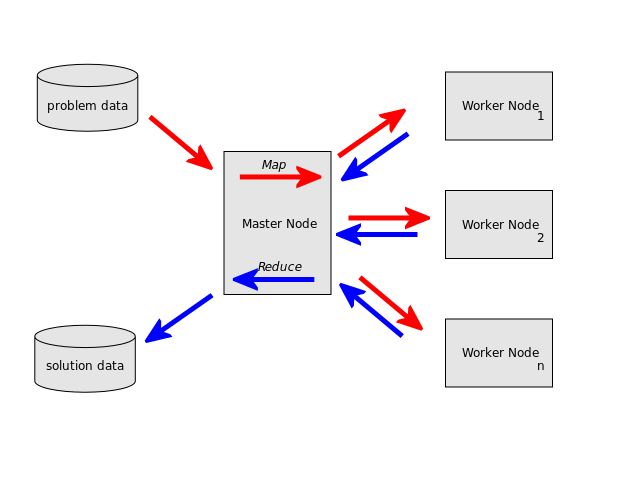
\includegraphics[width=0.6\textwidth]{Images/overview.png}
%   \caption{Solution Overview}
%   \label{fig:Scheme}
% \end{figure}


%%%%%%%%%%%%%%
% Evaluation %
%%%%%%%%%%%%%%
\section{Work Schedule}

A Gantt chart is shown in Figure~\ref{ganttchart}.

\begin{figure}
  \centering
  \rotatebox{90}{
    \tikzset{every picture/.style={xscale=0.8,yscale=0.8,transform shape}}
  \begin{ganttchart}[ y unit chart = 0.7cm,
      vgrid,
      bar top shift=-0.1,
      bar height=0.6,
      title height=0.7]{1}{36}
    \gantttitle{Feb'25}{4}
    \gantttitle{Mar'25}{4}
    \gantttitle{Apr'25}{4}
    \gantttitle{May'25}{4}
    \gantttitle{Jun'25}{4}
    \gantttitle{Jul'25}{4}
    \gantttitle{Aug'25}{4}
    \gantttitle{Sep'25}{4}
    \gantttitle{Oct'25}{4} \\
    \gantttitlelist{1,...,4}{1}
    \gantttitlelist{1,...,4}{1}
    \gantttitlelist{1,...,4}{1}
    \gantttitlelist{1,...,4}{1}
    \gantttitlelist{1,...,4}{1}
    \gantttitlelist{1,...,4}{1}
    \gantttitlelist{1,...,4}{1}
    \gantttitlelist{1,...,4}{1}
    \gantttitlelist{1,...,4}{1} \\

    \ganttgroup{Extend compiler features}{1}{7} \\
    \ganttbar{Code base clean-up}{1}{2} \\
    \ganttbar{Affine sessions and shared mutable state}{3}{5} \\
    \ganttbar{Native types}{6}{6} \\
    \ganttbar{C Interoperability}{7}{7} \\

    \ganttgroup{Profiling and optimization}{8}{23} \\
    \ganttbar{Run tests and evaluate solution}{8}{8}\\
    \ganttbar{Better memory management}{9}{11} \\
    \ganttbar{Multi-threading}{12}{12} \\
    \ganttbar{Investigate and implement other optimizations}{13}{23} \\

    \ganttgroup{Writing dissertation}{1}{36} \\
    \ganttbar{Alpha version}{1}{23} \\
    \ganttbar{Final revision by advisor}{24}{27} \\
    \ganttbar{Beta version}{28}{36} \\

  \end{ganttchart}
  }
  \caption{Planned Schedule}
  \label{ganttchart}
\end{figure}


%%%%%%%%%%%%%%%%%
% Work Schedule %
%%%%%%%%%%%%%%%%%
\section{Work Schedule}
% \lipsum[7]

A Gantt chart is shown in Figure~\ref{ganttchart}.

\begin{figure}
\centering
\rotatebox{90}{
\tikzset{every picture/.style={xscale=0.8,yscale=0.8,transform shape}}
\begin{ganttchart}[ y unit chart = 0.7cm,
                    vgrid, 
                    bar top shift=-0.1, 
                    bar height=0.6, 
                    title height=0.7]{1}{36}
  \gantttitle{Feb'19}{4}
  \gantttitle{Mar'19}{4}
  \gantttitle{Apr'19}{4}
  \gantttitle{May'19}{4} 
  \gantttitle{Jun'19}{4} 
  \gantttitle{Jul'19}{4} 
  \gantttitle{Aug'19}{4} 
  \gantttitle{Sep'19}{4} 
  \gantttitle{Oct'19}{4} \\
  \gantttitlelist{1,...,4}{1}
  \gantttitlelist{1,...,4}{1}
  \gantttitlelist{1,...,4}{1}
  \gantttitlelist{1,...,4}{1}
  \gantttitlelist{1,...,4}{1}
  \gantttitlelist{1,...,4}{1}
  \gantttitlelist{1,...,4}{1}
  \gantttitlelist{1,...,4}{1}
  \gantttitlelist{1,...,4}{1} \\
  
\ganttgroup{Study selected tools in more detail}{4}{12} \\
\ganttbar{Test selected tools}{4}{8} \\
\ganttbar{Evaluate results and select tool to extend}{9}{9} \\
\ganttbar{Deeper study of the selected tool}{10}{12} \\

\ganttgroup{Implementation}{13}{18} \\
\ganttbar{Extend selected tool}{13}{18} \\


\ganttgroup{Experimental evaluation}{19}{22} \\
\ganttbar{Run tests}{19}{20} \\
\ganttbar{Evaluate Solution}{21}{22} \\

\ganttgroup{Writing dissertation}{4}{36} \\
\ganttbar{Alpha version}{4}{24} \\
\ganttbar{Final revision by advisor}{25}{27} \\
\ganttbar{Beta version}{28}{36} \\

\end{ganttchart}
}
\caption{Planned Schedule}
\label{ganttchart}
\end{figure}


%%%%%%%%%%%%%%%%
% BIBLIOGRAPHY %
%%%%%%%%%%%%%%%%
\clearpage
% add Bibliography to TOC
\addcontentsline{toc}{section}{\refname}
% The following command resets the 'emphasis' style for bibliography entries
\normalem
% Name of your BiBTeX file
\bibliography{./Bibliography} % <-- ACTION: Put here your own filename or edit Bibliography.bib to add your references
% The following command modifies the 'emphasis' style for bibliography entries
\ULforem


%%%%%%%%%%%%
% APPENDIX %
%%%%%%%%%%%%
\clearpage % <-- ACTION: Comment the following blocks if you dont need appendixes
\appendix
\section{Title of Appendix}
This is an appendix.


%%%%%%%%%%%%%
%    END    %
%%%%%%%%%%%%%

\end{document}
